% This template stolen from Andrey Klitsunov. Thank you Andrew


\documentclass[14pt, a4paper]{extarticle}
\usepackage[utf8]{inputenc}
\usepackage[T2A]{fontenc}
\usepackage[russian]{babel}
\usepackage{setspace}
\usepackage{amssymb,amsfonts,amsmath,cite,enumerate,float,indentfirst}
\usepackage{mathrsfs}
\usepackage{comment}
\usepackage{verbatim}
\usepackage{url}
\usepackage{mathtools}
\usepackage[pdftex]{graphicx}
\usepackage{soul} 
\usepackage{titlesec}
\usepackage{hyperref}
\usepackage{gensymb}
% package for graph drawing
\usepackage{tikz}


% for custom captions
\usepackage{caption}
\DeclareCaptionLabelSeparator{ddash}{.---}
\captionsetup{labelsep=ddash}
\captionsetup[figure]{labelfont=bf}
\captionsetup[table]{justification=justified, singlelinecheck=false}

% for BDSM with table of contents
%\usepackage{tocloft}
%\renewcommand{\cftsecleader}{\cftdotfill{\cftdotsep}}

%\usepackage{tocstyle}
\usepackage{blindtext}


\usepackage{titletoc}%
\titlecontents{section}% <section-type>
[0pt]% <left>
{}% <above-code>
{\MakeUppercase\chaptername\ \thecontentslabel. }% <numbered-entry-format>
{}% <numberless-entry-format>
{\dotfill\contentspage}%

\titlecontents{subsection}% <section-type>
[0.8em]% <left>
{}% <above-code>
{\thecontentslabel. }% <numbered-entry-format>
{}% <numberless-entry-format>
{\dotfill\contentspage}%

% \dottedcontents{<section>}[<left>]{<above-code>}
% {<label width>}{<leader width>}
%\dottedcontents{section}[0em]{}{3.3em}{1pc}
%dottedcontents{subsection}[0em]{}{3.3em}{1pc}

%\usetocstyle{allwithdot}

% Redefinition of ToC command to get centered heading
\makeatletter
\renewcommand\tableofcontents{%
	\null\hfill\textbf{\large\contentsname}\hfill\null\par
	\@mkboth{\MakeUppercase\contentsname}{\MakeUppercase\contentsname}%
	\vspace{3em}%
	\@starttoc{toc}%
}
\makeatother


% also russian spacing
\singlespacing

% setting equation number
\renewcommand\theequation{\arabic{section}.\arabic{equation}}

\mathtoolsset{showonlyrefs=true} %equation number only for referenced

% smart tables
\usepackage{tabularx}
\usepackage{tabulary}

% smart ',' in math mode
%\usepackage{icomma}

% use to copy math sign to next line
\newcommand*{\hm}[1]{#1\nobreak\discretionary{}
	{\hbox{$\mathsurround=0pt #1$}}{}}

%redefining english style math symbols to russian style
\renewcommand{\epsilon}{\ensuremath{\varepsilon}}
\renewcommand{\phi}{\ensuremath{\varphi}}
\renewcommand{\kappa}{\ensuremath{\varkappa}}
\renewcommand{\le}{\ensuremath{\leqslant}}
\renewcommand{\leq}{\ensuremath{\leqslant}}
\renewcommand{\ge}{\ensuremath{\geqslant}}
\renewcommand{\geq}{\ensuremath{\geqslant}}
\renewcommand{\emptyset}{\varnothing}

% setting path to image folder
\graphicspath{{img/}}

% problem pasting command
% using style from Garey & Johnson
\newcounter{problem}[section]
\newcommand{\pasteproblem}[3]{
	\addtocounter{problem}{1}
	\noindent \textbf{\textsc{#1}} \\
	\noindent УСЛОВИЕ. #2\\
	\noindent ВОПРОС. #3\\
}

 % set page margins
\usepackage{geometry}
\geometry{left=3cm}
\geometry{right=1cm}
\geometry{top=2cm}
\geometry{bottom=2cm}

% set line space
\renewcommand{\baselinestretch}{1}
\setlength{\parskip}{0.8em}
\setlength{\parindent}{1.5em}

% set titles style
\usepackage{titlesec}
\titleformat{\section}[block]{\large\bfseries\center\onehalfspacing}{Глава \arabic{section}\\}{2pt}{}
\titleformat{\subsection}[block]{\large\bfseries}{\hspace{0.8em} \arabic{section}.\arabic{subsection} }{2pt}{}
\titleformat*{\subsubsection}{\bfseries}

% figure captions settings
\renewcommand\thefigure{\thesection.\arabic{figure}}  
\makeatletter
\renewcommand{\fnum@figure}{Рисунок \thefigure}
\makeatother

\makeatletter
\renewcommand\@biblabel[1]{#1.}
\makeatother

% table captions settings
\renewcommand\thetable{\thesection.\arabic{table}}  
\makeatletter
\renewcommand{\fnum@table}{Таблица \thetable}
\makeatother

% set theorems title style
\usepackage{amsthm}
\newtheorem{theorem}{Теорема}[section]
\newtheorem{corollary}{Следствие}[theorem]
\newtheorem{lemma}{Лемма}[section]
\newtheorem{statement}{Утверждение}[section]
\theoremstyle{remark}
\newtheorem{remark}{Замечание}[section]
\theoremstyle{definition}
\newtheorem{definition}{Определение}

% content title changing
\addto\captionsrussian{
  \renewcommand{\contentsname}
    {ОГЛАВЛЕНИЕ}
}

% bibliography title changing
\addto\captionsrussian{
  \renewcommand{\refname}
    {СПИСОК ЛИТЕРАТУРЫ}
}

\begin{document}
	\begin{titlepage}
    \begin{center}
      \textbf{ БЕЛОРУССКИЙ ГОСУДАРСТВЕННЫЙ УНИВЕРСИТЕТ}
    \end{center}
    
    \vspace{2em}
	\begin{flushleft}
		На правах рукописи \hspace{16em} \\
		УДК 004.852
	\end{flushleft}
	
	\vspace{2em}
	\begin{center}
		Песецкий Артем Степанович
	\end{center}
	\begin{center}
        {\bf Проблемные вопросы применения IT для решения задачи прогнозирования} \\
        \vspace{5mm}
        {Реферат по \\
        <<Основам информационных технолгий>>}
    \end{center}
	
	\vspace{2em}
	
	\hfill 
	\begin{minipage}{0.5\linewidth}
		Магистранта кафедры дискретной математики и алгоритмики факультета прикладной математики и информатики \\[0.5em]
		
		Специальность: 1-31 80 09 "--- прикладная математика и информатика \\[0.5em]
		
		Рецензент: \\
		Мамай Дарья Сергеевна
	\end{minipage}

    \vspace{8em}

    
    \vfill

    \begin{center}
        {\large \bf Минск, 2018}
    \end{center}
\end{titlepage}

	\setcounter{page}{2}
	\newpage
\tableofcontents
	\newpage
\section*{ВВЕДЕНИЕ}
\addcontentsline{toc}{section}{ВВЕДЕНИЕ}
В последние несколько лет все больше разнообразных повседневных задач решаются с помощью алгоритмов машинного обучения. Машинное обучение (англ. Machine Learning, ML) — класс методов искусственного интеллекта, характерной чертой которых является не прямое решение задачи, а обучение в процессе применения решений множества сходных задач. Для построения таких методов используются средства математической статистики, численных методов, методов оптимизации, теории вероятностей, теории графов, различные техники работы с данными в цифровой форме. Теоретические основы машинного обучения были заложены еще в середине прошлого века, однако в течение долгого времени эта область компьютерной науки практически не развивалась, так для использования алгоритмов машинного обучения необходимы были высокопроизводительные вычислительные системы. С достижением необходимой производительности в начале 2010-х алгоритмы машинного обучения стали все чаще использоваться в решении разнообразных практических задач, таких как распознавание речи, жестов и образов; техническая и медицинская диагностика, обнаружение спама и другие.  
Одной из областей машинного обучения являются алгоритмы прогнозирования. Приведем несколько примеров решенных задач прогнозирования и алгоритмов, применяемых для этого:
\begin{enumerate}
	\item
Прогнозирование финансовых процессов и биржевых индексов. В частности, Дегтярев В.М использовал многослойные нейронные сети для прогнозирования поведения валютной пары доллар США/ швейцарский франк и в результате построил модель для торговли на бирже, прибыль работы с при помощи которой составляла порядка 7 процентов \cite{one}. Также можно выделить работу Samuel Edet, который использовал рекуррентные нейронные сети для прогнозирования изменений значения индеков SA SnP 500\cite{two}. Точность полученной им модели составляла порядка 75 процентов.	
	\item
Медицинская диагностика. Примером работ в этой области можно привести можно привести работу сотрудников университета Стэнфорда, которые использовали сверточную нейронную сеть для прогнозирования возможной аритмии у пациентов по данным кардиограммы.\cite{cardio}
	\item
Спортивное прогнозирование. Алгоритмы машинного обучения использовались для прогнозирования результатов матчей в самых разных видах спорта. В частности, Kahn использовал многослойную нейронную сеть для построения модели классификации для прогнозирования результатов матчей NFL в 2003 году. В качестве обучающей выборки были использованы первые 192 матча сезона. В результате результаты прогноза модели превзошли результаты предсказаний профессиональных экспертов. \cite{four}
\end{enumerate}
В качестве задачи прогнозирования была выбрана задача теннисного прогнозирования.
\section*{ОСНОВНЫЕ ПОНЯТИЯ И ОПРЕДЕЛЕНИЯ}
\addcontentsline{toc}{section}{Основые определения и понятия}
Машинное обучение (англ. machine learning, ML) — класс методов искусственного интеллекта, характерной чертой которых является не прямое решение задачи, а обучение в процессе применения решений множества сходных задач. Для построения таких методов используются средства математической статистики, численных методов, методов оптимизации, теории вероятностей, теории графов, различные техники работы с данными в цифровой форме.

Теннис — это игра с ракеткой, в которую могут играть как один на один, так и парами. Для простоты сфокусируемся на предсказании результатов одиночных матчей. Дадим определение задачи теннисного прогнозирования.Пусть имеется следующая информация о предстоящем теннисном матче: имена участников, тип покрытия и позиции игроков в рейтинге ATP; а также историческая информация об уже сыгранных матчах. Необходимо построить модель на основе исторических данных, которая будет наилучшим образом прогнозировать результаты предстоящих матчей. Выбор данной задачи был сделан по нескольким причинам. Во-первых, теннис является одним из самых популярных видов спорта, а рынок ставок на теннис является одним из крупнейших. Во-вторых, на данный момент большинство средств для решения данной задачи используют в своей основе статистические модели, а алгоритмы машинного обучения для этой задачи практически не используются.

Обучающая выборка - набор данных для построения, обучения и анализа алгоритма машинного обучения. В случае задачи теннисного прогнозирования данная выборка представлена ранее сыгранными теннисными матчами и информацией о них.


	\newpage
\section{ИНСТРУМЕНТЫ ДЛЯ АНАЛИЗА И ОБРАБОТКИ ДАННЫХ}

\subsection{Общая схема решения задачи прогнозирования}
Приведем шаги для решения задачи прогнозирования:
\begin {enumerate}
	\item Поиск и фильтрация данных, построение обучающей выборки;
	\item Отбор наиболее релевантных признаков для построения обучающей выборки;	
	\item Построение и обучение модели;
	\item Анализ полученных результатов.
\end{enumerate}

В качестве языка программирования был использован Python. Python — высокоуровневый язык программирования общего назначения, ориентированный на повышение производительности разработчика и читаемости кода. Синтаксис ядра Python минималистичен. В то же время стандартная библиотека включает большой объём полезных функций. Python поддерживает несколько парадигм программирования, в том числе структурное, объектно-ориентированное, функциональное, императивное и аспектно-ориентированное. Основные архитектурные черты — динамическая типизация, автоматическое управление памятью, полная интроспекция, механизм обработки исключений, поддержка многопоточных вычислений и удобные высокоуровневые структуры данных. Код в Python организовывается в функции и классы, которые могут объединяться в модули (они в свою очередь могут быть объединены в пакеты).

Выбор в пользу данного языка был обусловлен наличием на нем большого количества библиотек, предназначенных для разработки и обучения алгоритмов машинного обучения. Важным преимуществом этих библиотек является наличие имплементаций низкоуровневых операций на языке С, что благоприятно влияет на производительность. 

Проведем обзор иструментов и библиотек, которые были использованы для решения поставленных выше задач.

\subsection{Построение обучающей выборки}
Для построения обучающей выборки из источника 1 была загружена информация об мужских одиночных теннисных матчах, сыгранных под эгидой ATP, за 2004-2018 годы. Для фильтрации данных и построения выборки использовался фреймворк Pandas.

Pandas – библиотека языка Python, предназначенная для обработки и анализа данных. Работа библиотеки построена поверх библиотеки NumPy. Библиотекой предоставляются разнообразные структуры и алгоритмы числовыми данными и временными рядами. Дадим краткое описание возможностей библиотеки:
\begin{itemize}
	\item
объект DataFrame, позволяющий манипулировать индексированными двумерными данными;
	\item
возможность обмена файлами разнообразных типов, а также между структурами в оперативной памяти;
	\item
наличие инструментов объединения данных, а также возможность обработки недостающей информации;
	\item
переформатирование информации, в том числе создание сводных таблиц данных;
	\item
наличие возможности получения среза данных по индексу, возможность получения выборки из больших объемов информации.\cite{five}
\end{itemize}

\subsection{Отбор признаков. Построение и обучение алгоритмов.}
После построения набора признаков для каждого из матча полученной обучающей выборки из него с помощью были выбраны наиболее релевантные признаки. Для этого реализация алгоритма RFE(recursive feature elimination) из библиотеки Scikit-learn.

Scikit-learn – библиотека для машинного обучения, написанная на языке Python.  В нее включены разнообразные алгоритмы классификации, регрессии и кластеризации, такие как случайный лес, метод опорных векторов, k-means, DBSCAN и другие. Разработка библиотеки началась Дэвидом Корнапеу в рамках проекта Google Summer of Code. Позже оригинальная кодовая база была полностью переписана другими разработчиками. Релиз библиотеки состоялся в феврале 2010 года после того, как в проект включились студенты французского государственного института исследований в информатике и автоматике INRIA. На данный момент данная библиотека завоевала популярность, и разработка обновлений продолжается. Основная часть кодовой базы написана на Python, часть алгоритмов написана на Cython для достижения большей производительности. Поддержка метода нелинейных опорных векторов реализована с помощью обертки на Cython вокруг библиотеки LIBSVM, а поддержка линейной регрессии и линейного метода опорных векторов с помощью обертки вокруг библиотеки LIBLINEAR. В данной работе эта библиотека использовалась для построения моделей логистической регрессии и метода опорных векторов, а также для отбора наиболее релевантных признаков с помощью алгоритма RFE.

После получения набора наиболее релевантных признаков с их помощью были построены 3 модели на основании следующих алгоритмов:
\begin{itemize}
\item
логистическая регрессия - это статистическая модель, используемая для предсказания вероятности возникновения некоторого события путём подгонки данных к логистической кривой?;
\item
искусственная нейронная сеть (ИНС) — математическая модель, а также её программное или аппаратное воплощение, построенная по принципу организации и функционирования биологических нейронных сетей — сетей нервных клеток живого организма. Это понятие возникло при изучении процессов, протекающих в мозге, и при попытке смоделировать эти процессы;
\item
метод опорных векторов (англ. SVM, support vector machine) — набор схожих алгоритмов обучения с учителем, использующихся для задач классификации и регрессионного анализа. Принадлежит семейству линейных классификаторов и может также рассматриваться как специальный случай регуляризации по Тихонову. Особым свойством метода опорных векторов является непрерывное уменьшение эмпирической ошибки классификации и увеличение зазора, поэтому метод также известен как метод классификатора с максимальным зазором.
\end{itemize}

Для построения указанных алгоритмов использовалась выше описанная библиотека Scikit-learn, а также библиотека Keras.

Keras – открытая библиотека на языке Python, предназначенная для построения нейросетевых моделей. Представляет собой интерфейс, надстроенный над Deeplearning4j, TensorFlow и Theano. Основным предназначением библиотеки является работа с нейронными сетями глубокого обучения. Библиотека было представлена в рамках проекта ONEIROS. Основным автором библиотеки является инженер Google Франсуа Шолле. Keras содержит в себе все основные реализации широко применяемых при создании нейронных сетей элементов, такие как слои, целевые и передаточные функции, оптимизаторы, а также набор инструментов для упрощения работы с картинками и текстом. Исходный код библиотеки размещен в открытом репозитории на Github. В работе данная модель использовалась для построения и обучения нейронной сети.

Для демострации работы моделей необходимо построить программу с графическим интерфейсом. Для его построения была использована библиотека Qt. Qt — кроссплатформенный фреймворк для разработки программного обеспечения на языке программирования C++. Есть также «привязки» ко многим другим языкам программирования: Python — PyQt, PySide; Ruby — QtRuby; Java — Qt Jambi; PHP — PHP-Qt и другие.

Со времени своего появления в 1996 году библиотека легла в основу многих программных проектов. Кроме того, Qt является фундаментом популярной рабочей среды KDE, входящей в состав многих дистрибутивов Linux.

Qt позволяет запускать написанное с его помощью программное обеспечение в большинстве современных операционных систем путём простой компиляции программы для каждой системы без изменения исходного кода. Включает в себя все основные классы, которые могут потребоваться при разработке прикладного программного обеспечения, начиная от элементов графического интерфейса и заканчивая классами для работы с сетью, базами данных и XML. Является полностью объектно-ориентированным, расширяемым и поддерживающим технику компонентного программирования.

Отличительная особенность — использование метаобъектного компилятора — предварительной системы обработки исходного кода. Расширение возможностей обеспечивается системой плагинов, которые возможно размещать непосредственно в панели визуального редактора. Также существует возможность расширения привычной функциональности виджетов, связанной с размещением их на экране, отображением, перерисовкой при изменении размеров окна.

\subsection{Выводы}
Средства языка Python, а также дополнительные библиотеки такие как Pandas, Scikit-lear, Keras и QT позволяют эффективно строить модели на основе алгоритмов машинного обучения для решения разнообразных задач прогнозировани, а также графический интерфейс для демонстрации работы полученных моделей.


	\newpage
\section{СРЕДСТВА ДЛЯ НАПИСАНИЯ КОДА И НАПИСАНИЯ РАБОТЫ}
\subsection{Средства для написания кода}
Cамыми популярными средами написания кода на языке программирования Python являются следующие IDE(англ. Integrated Development Environment - интегрировання среда разработки): IntelliJ IDEA PyCharm, Jupiter Notebook расширение для IPython и Spyder.

PyCharm — интегрированная среда разработки для языка программирования Python. Предоставляет средства для анализа кода, графический отладчик, инструмент для запуска юнит-тестов и поддерживает веб-разработку на Django. PyCharm разработана компанией JetBrains[5] на основе IntelliJ IDEA. PyCharm работает под операционными системами Windows, Mac OS X и Linux. PyCharm Professional Edition имеет несколько вариантов лицензий, которые отличаются функциональностью, стоимостью и условиями использования.PyCharm Professional Edition является бесплатным для образовательных учреждений и проектов с открытым исходным кодом.Существует также бесплатная версия Community Edition, обладающая усеченным набором возможностей. Распространяется под лицензией Apache 2.

Ключевые возможности PyCharm:
\begin{itemize}
	\item статический анализ кода, подсветка синтаксиса и ошибок.
	\item навигация по проекту и исходному коду: отображение файловой структуры проекта, быстрый переход между файлами, классами, методами и использованиями методов.
	\item рефакторинг: переименование, извлечение метода, введение переменной, введение константы, подъём и спуск метода и т. д.
	\item инструменты для веб-разработки с использованием фреймворка Django
	\item встроенный отладчик для Python
	\item встроенные инструменты для юнит-тестирования
	\item разработка с использованием Google App Engine
	\item поддержка систем контроля версий: общий пользовательский интерфейс для Mercurial, Git, Subversion, Perforce и CVS с поддержкой списков изменений и слияния.
\end{itemize}

Spyder (ранее Pydee) — свободная и кроссплатформенная интерактивная IDE для научных расчетов на языке Python, обеспечивающая простоту использования функциональных возможностей и легковесность программной части. Spyder является частью модуля spyderlib для Python, основанного на PyQt4, pyflakes, rope и Sphinx, предоставляющего мощные виджеты на PyQt4, такие как редактор кода, консоль Python (встраиваемая в приложения), графический редактор переменных (в том числе списков, словарей и массивов).

Ключевые возможности Spyder:
\begin{itemize}
	\item редактор с подсветкой синтаксиса Python, C/C++ и Fortran
	\item динамическая интроспекция кода (с помощью rope) — автодополнение, переход к определению объекта по клику мыши
	\item нахождение ошибок на лету (с использованием pyflakes)
	\item поддержка одновременного использования множества консолей Python (включая оболочку IPython)
	\item просмотр и редактирование переменных с помощью GUI (поддерживаются различные типы данных - числа, строки, списки, массивы, словари)
	\item встроенные средства доступа к документации (в формате Sphinx)
	\item гибко настраиваемый интерфейс
	\item интеграция с научными библиотеками Python - NumPy, SciPy, Matplotlib, Pandas.
\end{itemize}

IPython (англ. Interactive Python) — интерактивная оболочка для языка программирования Python, которая предоставляет расширенную интроспекцию, дополнительный командный синтаксис, подсветку кода и автоматическое дополнение. Является компонентом пакетов программ SciPy и Anaconda. IPython позволяет осуществлять неблокирующее (англ. non-blocking) взаимодействие с Tkinter, GTK, Qt и WX. Стандартная библиотека Python включает лишь Tkinter. IPython может интерактивно управлять параллельными кластерами, используя асинхронные статусы обратных вызовов и/или MPI. IPython может использоваться как замена стандартной командной оболочки операционной системы, особенно на платформе Windows, возможности оболочки которой ограничены. Поведение по умолчанию похоже на поведение оболочек UNIX-подобных систем, но тот факт, что работа происходит в окружении Python, позволяет добиваться большей настраиваемости и гибкости.
Начиная с версии 4.0, монолитный код был разбит на модули, и независимые от языка модули были выделены в отдельный проект Jupyter. Наиболее известной веб-оболочкой для IPython является Jupyter Notebook (ранее известный как IPython Notebook), позволяющая объединить код, текст и диаграммы, и распространять их для других пользователей.

Для хранения исходного кода была использована система контроля версий Git. Git — распределённая система управления версиями. Проект был создан Линусом Торвальдсом для управления разработкой ядра Linux, первая версия выпущена 7 апреля 2005 года. На сегодняшний день его поддерживает Джунио Хамано. Среди проектов, использующих Git — ядро Linux, Swift, Android, Drupal, Cairo, GNU Core Utilities, Mesa, Wine, Chromium, Compiz Fusion, FlightGear, jQuery, PHP, NASM, MediaWiki, DokuWiki, Qt, ряд дистрибутивов Linux.Программа является свободной и выпущена под лицензией GNU GPL версии 2. По умолчанию используется TCP порт 9418.

Система спроектирована как набор программ, специально разработанных с учётом их использования в сценариях. Это позволяет удобно создавать специализированные системы контроля версий на базе Git или пользовательские интерфейсы. Например, Cogito является именно таким примером оболочки к репозиториям Git, а StGit использует Git для управления коллекцией исправлений (патчей).Git поддерживает быстрое разделение и слияние версий, включает инструменты для визуализации и навигации по нелинейной истории разработки. Как и Darcs, BitKeeper, Mercurial, Bazaar и Monotone[en], Git предоставляет каждому разработчику локальную копию всей истории разработки, изменения копируются из одного репозитория в другой.Удалённый доступ к репозиториям Git обеспечивается git-демоном, SSH- или HTTP-сервером. TCP-сервис git-daemon входит в дистрибутив Git и является наряду с SSH наиболее распространённым и надёжным методом доступа. Метод доступа по HTTP, несмотря на ряд ограничений, очень популярен в контролируемых сетях, потому что позволяет использовать существующие конфигурации сетевых фильтров.

\subsection{Средства для написания реферата}
В качестве системы текстовой верстки был использован Latex. Latex — наиболее популярный набор макрорасширений (или макропакет) системы компьютерной вёрстки TeX, который облегчает набор сложных документов. В типографском наборе системы TeX форматируется традиционно как Latex.

Пакет позволяет автоматизировать многие задачи набора текста и подготовки статей, включая набор текста на нескольких языках, нумерацию разделов и формул, перекрёстные ссылки, размещение иллюстраций и таблиц на странице, ведение библиографии и др. Кроме базового набора существует множество пакетов расширения Latex. Первая версия была выпущена Лесли Лэмпортом в 1984 году; текущая версия, Latex2e, после создания в 1994 году испытывала некоторый период нестабильности, окончившийся к концу 1990-х годов, а в настоящее время стабилизировалась (хотя раз в год выходит новая версия).

Общий внешний вид документа в LaTeX определяется стилевым файлом. Существует несколько стандартных стилевых файлов для статей, книг, писем и т. д., кроме того, многие издательства и журналы предоставляют свои собственные стилевые файлы, что позволяет быстро оформить публикацию, соответствующую стандартам издания.

Возможности системы, не ограничены, благодаря механизму программирования новых макросов. Вот список некоторых возможностей, предлагаемых стандартными макросами и теми, которые можно скачать с сервера CTAN:
\begin{itemize}
	\item алгоритмы расстановки переносов, определения междусловных пробелов, балансировки текста в абзацах;
	\item автоматическая генерация содержания, списка иллюстраций, таблиц и т. д.;
	\item механизм работы с перекрёстными ссылками на формулы, таблицы, иллюстрации, их номер или страницу;
	\item механизм цитирования библиографических источников, работы с библиографическими картотеками;
	\item размещение иллюстраций (иллюстрации, таблицы и подписи к ним автоматически размещаются на странице и нумеруются);
	\item оформление математических формул, возможность набирать многострочные формулы, большой выбор математических символов;
	\item оформление химических формул и структурных схем молекул органической и неорганической химии;
	\item оформление графов, схем, диаграмм, синтаксических графов;
	\item оформление алгоритмов, исходных текстов программ (которые могут включаться в текст непосредственно из своих файлов) с синтаксической подсветкой;
	\item разбивка документа на отдельные части (тематические карты).
\end{itemize}
Расширенные средства работы с библиографическими данными предоставляются программой BibTeX. Базовые возможности работы с математическими формулами расширяются с помощью пакета AMS-LaTeX.

\subsection{Выводы}
Современные интегрированные среды разработки вкупе с системой контроля версий позволяют эффективно использовать средства языка Python  и дополнительных библиотек при разработки моделей алгоритмов для машинного обчуения.

Текствоый процессор Latex позволяет эффективно создавать и форматировать документы.
	\newpage\section*{ЗАКЛЮЧЕНИЕ}\addcontentsline{toc}{section}{ЗАКЛЮЧЕНИЕ}
В реферате были изучены програмные средства и библиотеки, которые могут применяться для построения моделей машинного обучения, решающих задачу прогнозирования.Использование описанных алгоритмов и программных средств позволило построить модели, решающие задачу теннисного прогнозирования.Точность полученных моделей составила порядка 75 процентов.

Использование современных интегрированных сред разработки, таких как PyCharm, Spyder и Jypiter Notebook позволяют эффективно отбирать данные, строить алгоритмы на их основе, а также эффективно анализировать и визуализировать данные. Имользование системы контроля версий Git позволяет удобно следить за историй изменения програмного кода, а также коллаборироваться с другими исследователями. 

Система коипютерной верстки TeX, в частности ее набор макрорасширений Latex позволяют быстро создавать текстовые документы с вставкой в них  математических и химических формул, графиков, таблиц и других мультимедийных элементов.


	\newpage
\begin{thebibliography}{3}
	\addcontentsline{toc}{section}{СПИСОК ЛИТЕРАТУРЫ}
	\bibitem{one}В. Дегтярев. Прогнозирование валютных курсов с использованием эконометрических моделей и искусственных нейронных сетей: дис. : Дегтярев В. М – 2012 – 103с.
	
	\bibitem{two}Recurrent Neural Networks in Forecasting SnP 500 Index // Научный портал https://papers.ssrn.com/ [Электронный ресурс]. – 2017. - Режим доступа: https://papers.ssrn.com/sol3/papers.cfm?abstractid=3001046 - Дата доступа: 04.05.2018.
	
	\bibitem{cardio}Cardiologist-Level Arrhythmia Detection with Convolutional Neural Networks. // Интернет-портал Cournell University Library [Электронный ресурс]. – 2017. - Режим доступа: https://arxiv.org/abs/1707.01836 - Дата доступа: 04.05.2018.
	
	\bibitem{four}J. Kahn. Neural network prediction of NFL football games / J. Kahn. // World Wide Web Electronic Publication. -  2003 – P. 9 – 15.
	
	\bibitem{five} Pandas package overview // Информационный портал http://pandas.pydata.org/ [Электронный ресурс]. – 2018. - Режим доступа: http://pandas.pydata.org/pandas-docs/stable/overview.html - Дата доступа: 04.11.2018.
	
\end{thebibliography}
	\newpage
\newpage\section*{ПРИЛОЖЕНИЯ}\addcontentsline{toc}{section}{ПРИЛОЖЕНИЯ}
\section*{Приложение A}
\section*{Сайт}
https://shogifun.github.io/

\begin{figure}[h]
	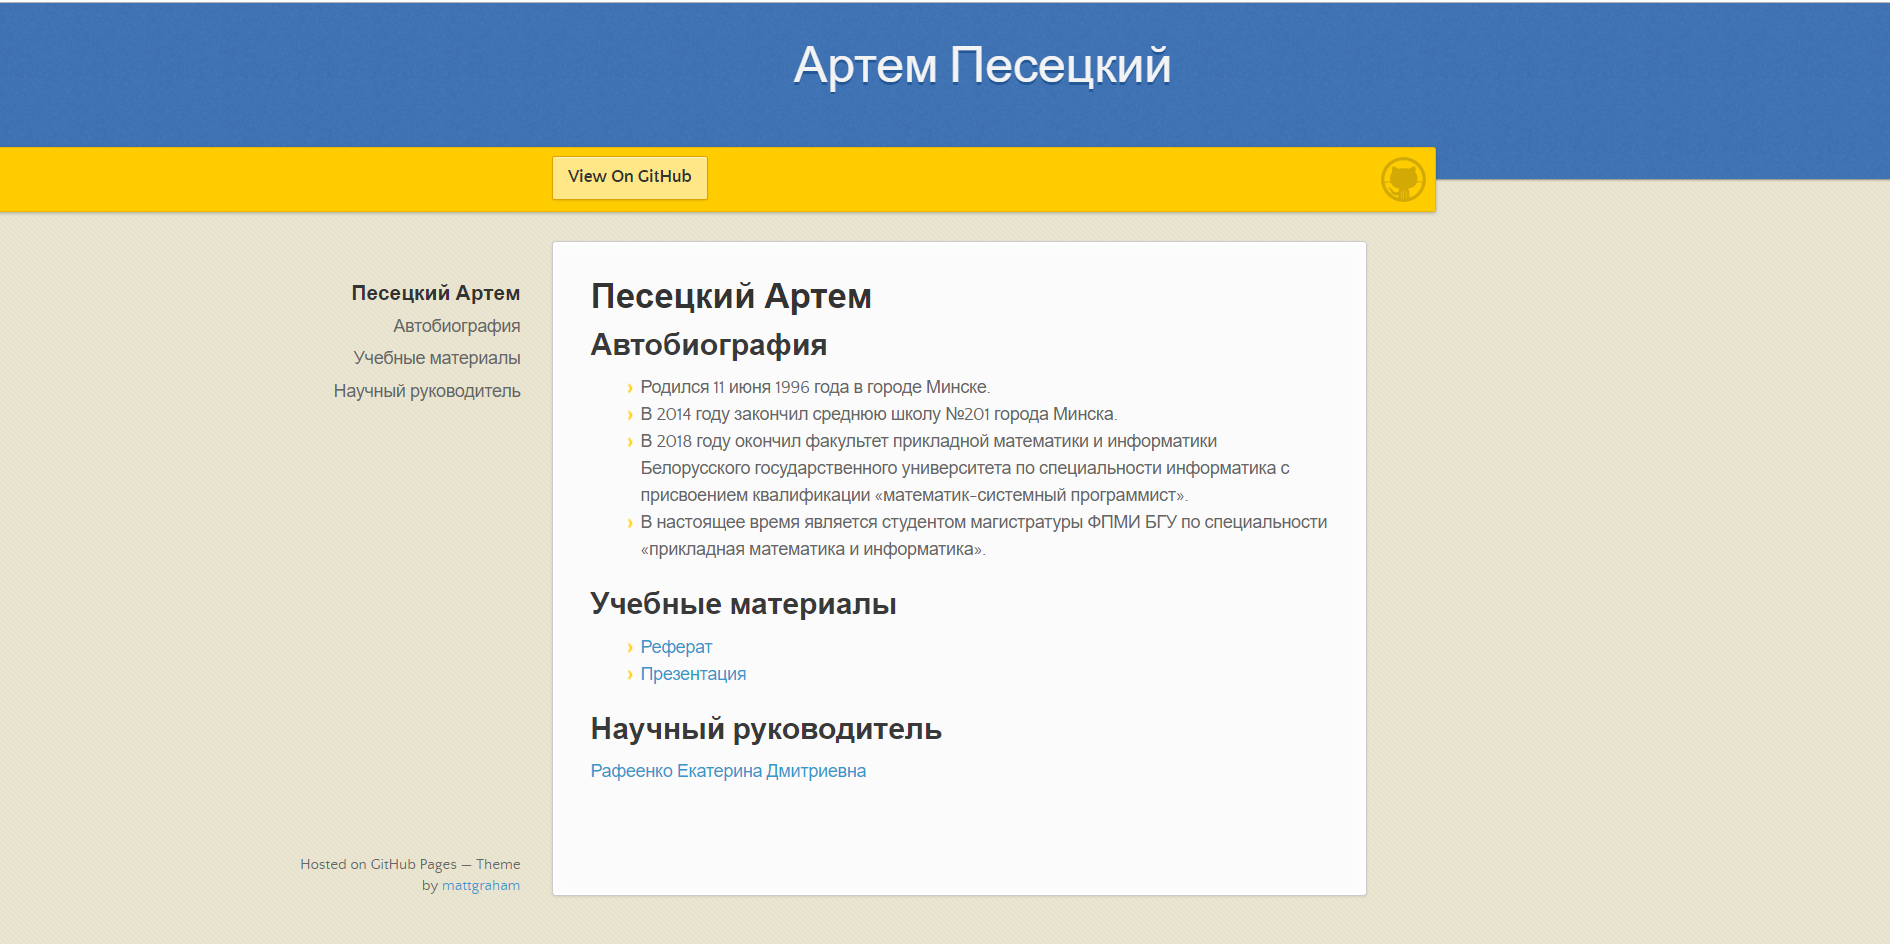
\includegraphics[scale=0.5]{images/site.png}
\end{figure}
	\newpage
\section*{Приложение B}
\section*{Презентация}
\begin{figure}[h]
	
\includegraphics[scale=0.5]{images/1.JPG}
	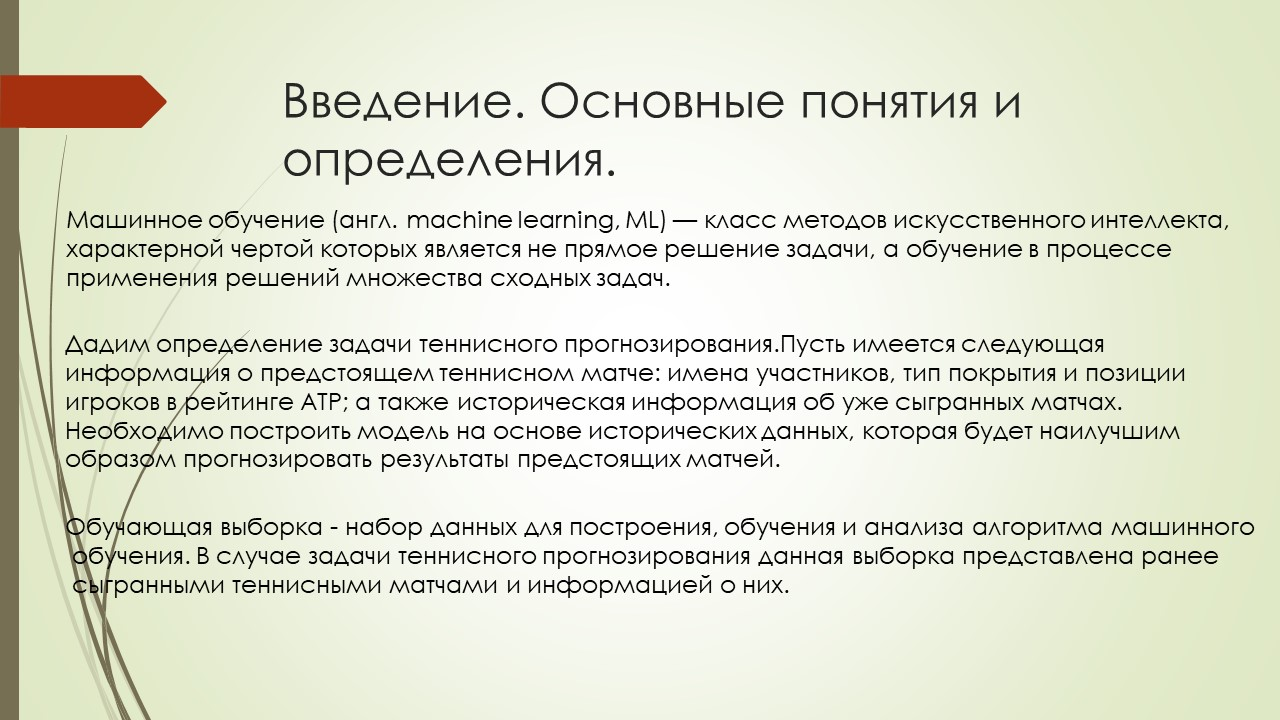
\includegraphics[scale=0.5]{images/2.JPG}
\end{figure}
\begin{figure}[h]
	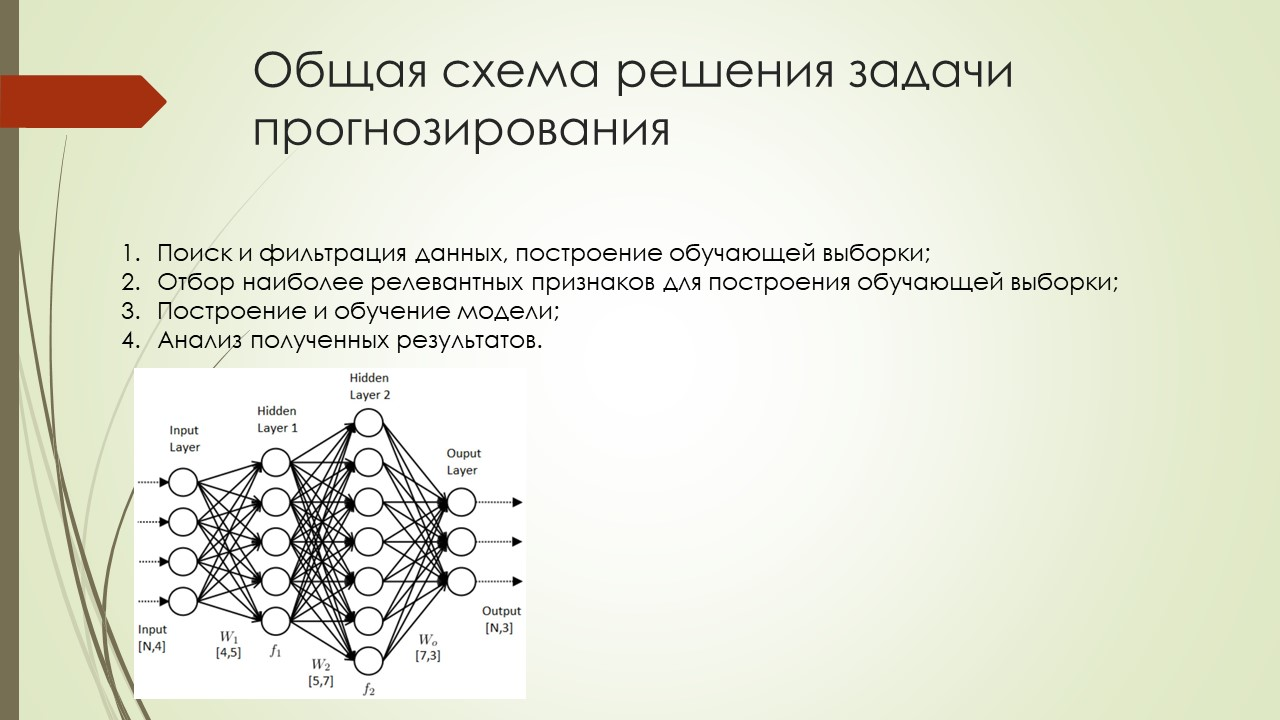
\includegraphics[scale=0.5]{images/3.JPG}
	
\includegraphics[scale=0.5]{images/4.JPG}
\end{figure}
\begin{figure}[h]
	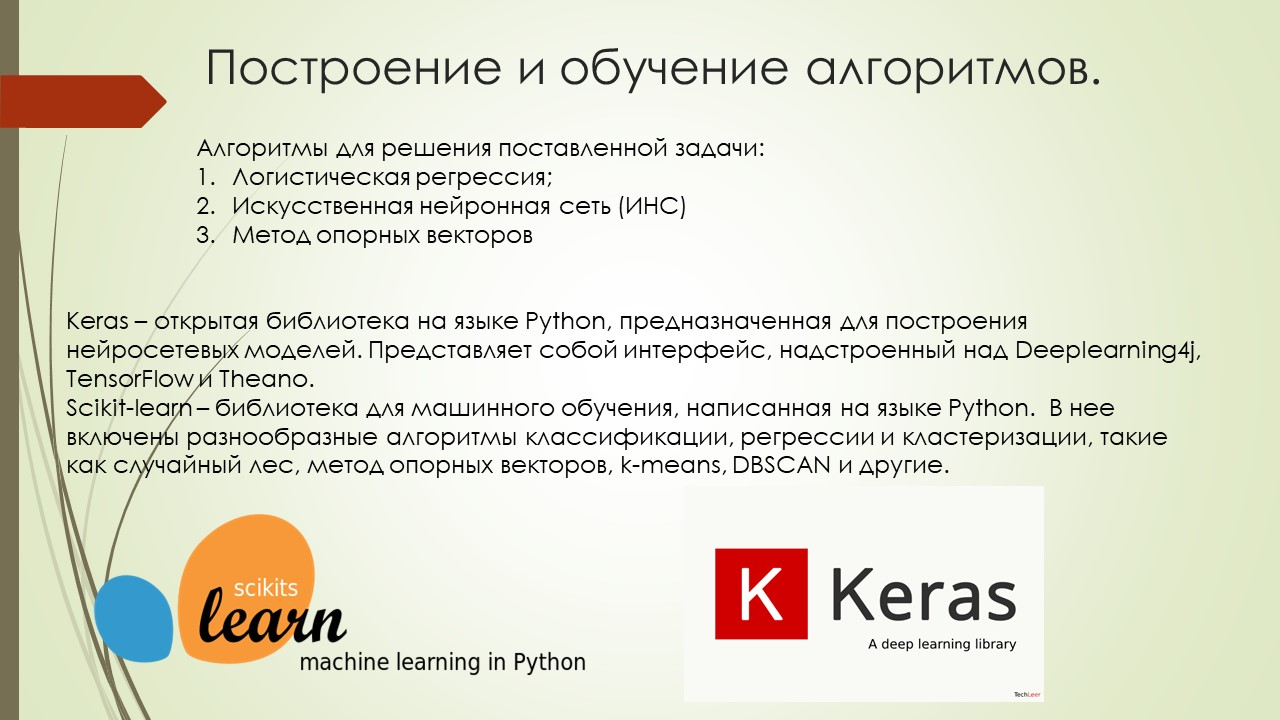
\includegraphics[scale=0.5]{images/5.JPG}
	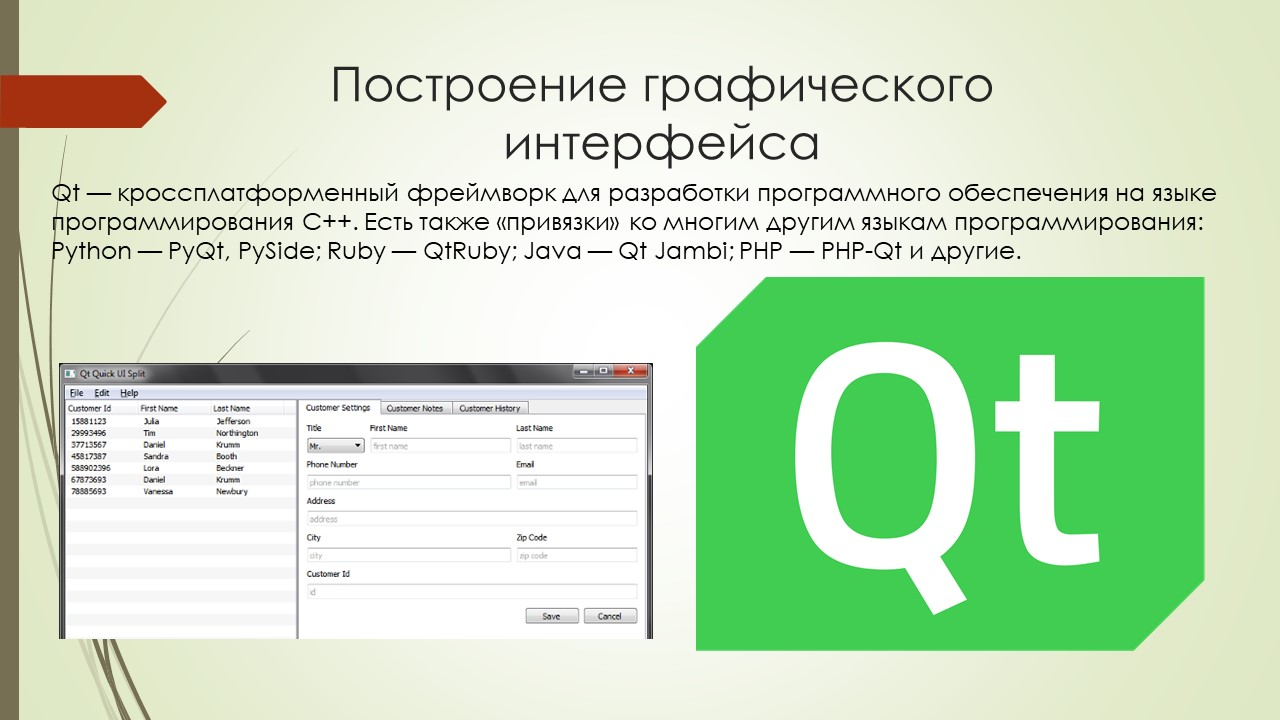
\includegraphics[scale=0.5]{images/6.JPG}
\end{figure}
\begin{figure}[h]
	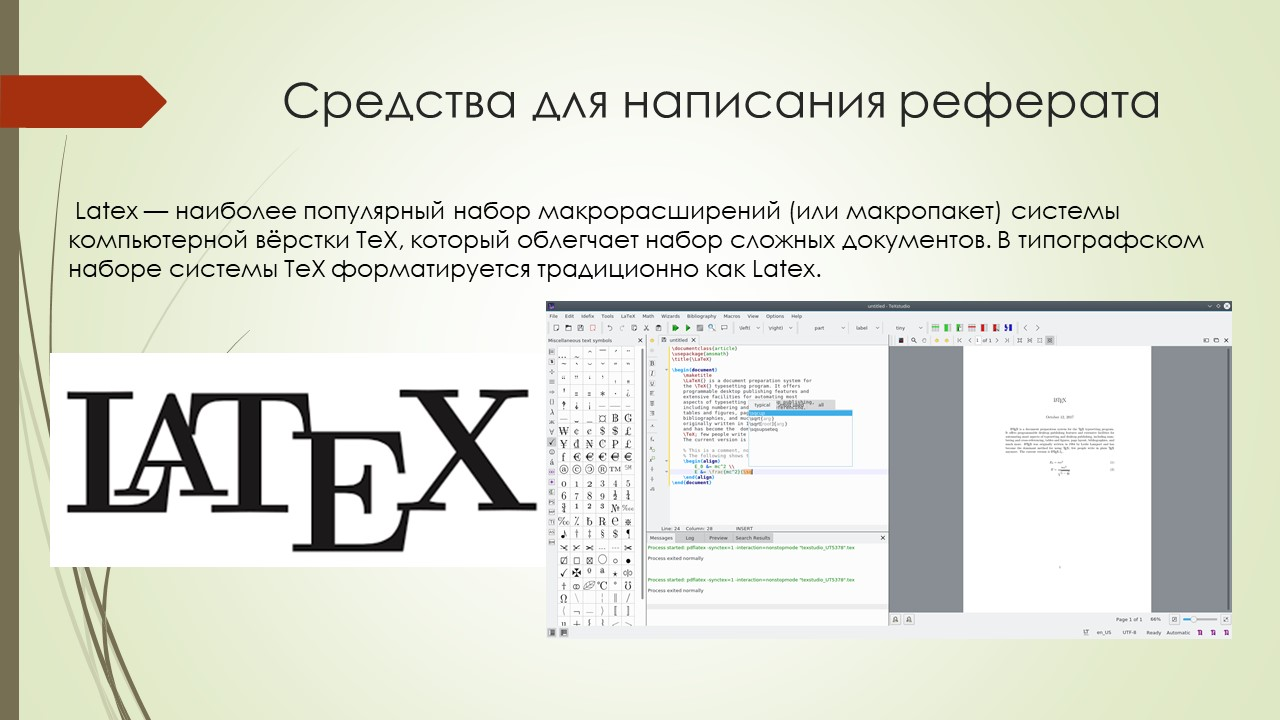
\includegraphics[scale=0.5]{images/7.JPG}
\end{figure}
\end{document}

